\documentclass[12pt,preprint]{aastex}

\newcommand{\vdag}{(v)^\dagger}
\newcommand{\myemail}{skywalker@galaxy.far.far.away}
\slugcomment{Draft version}
 
\shorttitle{A Study of the Point Spread Function at SDSS}
\shortauthors{Xin, Ivezi\'{c} and Friends}
 
\begin{document}

\title{A Study of the Point Spread Function in SDSS Images}    %line break \\ is allowed in title

\author{B. Xin$^1$, \v{Z}. Ivezi\'{c}$^2$, R.H. Lupton$^3$, P. Yoachim$^2$, R.L. Jones$^2$, C. Claver$^1$, G. Angeli$^1$}
\and
\author{Other Contributors}

\affil{$^1$Large Synoptic Survey Telescope, Tucson, AZ 85719}
\affil{$^2$Department of Astronomy, University of Washington, Seattle, WA 98195}
\affil{$^3$Department of Astrophysical Sciences, Princeton University, Princeton, NJ 08544}

\begin{abstract}
We use SDSS imaging data in $ugriz$ passbands to study the shape of
point spread function (PSF) profile and the variation of its width with 
wavelength and time. We find that the PSF profile is well described by 
theoretical predictions based on von Karman's turbulence theory and
can be parametrized by two parameter, the profile's FWHM (full width
at half maximum) and a normalization on a empirical instrumental PSF. 
The profile shape is very similar to the ``double gaussian
plus power-law wing'' decomposition used by SDSS, but here it is modeled 
with two free model parameter, rather than six as in SDSS pipeline. 
The FWHM variation with wavelength folows the
$\lambda^{\alpha}$ power law, where $\alpha \approx-0.3$, and is correlated
with the FWHM itself. We also measure the temporal and angular
structure functions for FWHM and compare them to simulations and
existing measurements.
\end{abstract}

\keywords{imaging point spread function --- SDSS}
 


\section{Introduction}


% \section{Introduction}

ZI write a brief overview of SDSS and motivation for analysis (e.g. performance optimization
for LSST, \citealt{LSSToverview}): this shouldn't be hard and can be done in about a day. 

Hey Bo! Here is an example of using bibtex and cite call: SDSS PSF algorithm is described 
in \cite{Lupton2001}, \cite{Lupton2002}, and \citet[][see \S4.3]{SDSSEDR}.

Bo or ZI: add a brief summary with a few references (e.g. Young, Tyson, Roddier,
Tokovinin papers; can also recruit George for this part!) about what is known 
regarding:  PSF profile shape (e.g. Kolmogorov vs. von Karman), 
the dependence of FWHM on wavelength, and angular and temporal 
structure functions. 

Paper layout here.

  

\section{Data Overview} 


%\section{Data Overview} 

We describe here the SDSS dataset and seeing estimates used in this work. The
selected subset of data, the so-called Stripe 82, represents about one third of
all SDSS imaging data. 

\subsection{Stripe 82 dataset} 

The equatorial Stripe 82 region (22$^h$24$^m$ $<$ R.A. $<$ 04$^h$08$^m$, 
$-$1.27$^\circ$  $<$ Dec $<$ $+$1.27$^\circ$, about 
290 deg$^2$) from the southern Galactic cap ($-64^\circ < b <  -20^\circ$) was repeatedly imaged (of order
one hundred times) by SDSS to study time-domain phenomena (such as supernovae, asteroids, variable stars, quasar 
variability).  An observing stretch of SDSS imaging data is called a ``run''. Often there is only a single
run for a given observing night, though sometimes there are multiple
runs per night. In this paper we use seeing data for 
108 runs, with a total of 947,400 fields, obtained between September,
1998 and September 2008 (there are 6 camera columns, each with 5 filters; for more
details please see \citealt{Gunn2006}). All runs are obtained during the Fall observing season (September to 
December). Astrometric and photometric aspects of this dataset have been discussed in detail by 
\cite{Ivezic2007} and \cite{Sesar2007}. 


\subsection{The treatment of seeing in SDSS}
 
Even in the absence of atmospheric inhomogeneities, the SDSS telescope delivers images whose 
FWHMs vary by up to 15\% from one side of a CCD to the other; the worst effects are seen in 
the chips farthest from the optical axis \citep{Gunn2006}. Moreover, since the atmospheric 
seeing varies with time, the delivered image quality is a complex two-dimensional function 
even on the scale of a single field (for an example of the instantaneous image quality across 
the imaging camera, see Figure 7 in \citealt{SDSSEDR}). 
 
The SDSS imaging PSF is modeled 
heuristically in each band using a Karhunen-Lo\'{e}ve (K-L) transform \citep{Lupton2002}. 
Using stars brighter than roughly 20$^{th}$ magnitude, the PSF images from a series of five 
fields are expanded into eigenimages and the first three terms are kept (K-L transform is 
also known as the Principal Component Analysis). The angular variation of the eigencoefficients
is fit with polynomials, using data from the field in question, plus the immediately preceding 
and following half-fields. The success of this K-L expansion is gauged by comparing PSF 
photometry based on the modeled K-L PSFs with large-aperture photometry for the same 
(bright) stars \citep{SDSSEDR}. 
Parameters that characterize seeing for one field of imaging data are stored in the so-called psField 
files\footnote{https://data.sdss.org/datamodel/files/PHOTO\_REDUX/RERUN/RUN/objcs/CAMCOL/psField.html}. 
The status parameter flag for each field indicates the success of the K-L decomposition.

In addition to the K-L decomposition, the SDSS processing pipeline computes parameters of the 
best-fit circular double Gaussian, evaluated at the center of each field. The measured PSF profiles are 
extended to $\sim$30 arcsec using observations of bright stars and at such large radii 
double Gaussian fits underpredict the measured profiles. For this reason, the fits are extended 
to include the so-called ``power-law wings'', which is reminiscent of
the Moffat function,
\begin{equation}
\label{eq:SDSSPSF}
        PSF(r) = {\exp(-{r^2\over 2\,\sigma_1^2}) + b\,\exp(-{r^2\over 2\,\sigma_2^2})
           + p_0\left(1 + { r^2 \over \beta \sigma_P^2}\right)^{-\beta/2} \over 1 + b + p_0}.
\end{equation} 
The measured PSFs are thus modeled using 6 free parameters ($\sigma_1$, $\sigma_2$, $\sigma_P$,
$b$, $p_0$ and $\beta$), and the best-fit parameters are reported in the psField files. 
Given that the measured profiles include only up to 10 data points, the fits are usually excellent
although they do not appear very robust (for examples of bad fits see Sec.~\ref{sec:psffit}).
%Fig.~\ref{fig:psffit}). 

 


\section{The PSF profile analysis}


%  \section{The PSF profile analysis}

Since the complex 6-parameter PSF fit given by Eq.~(\ref{eq:SDSSPSF}) was adopted by 
the SDSS processing pipeline, significant progress has been made in validating the 
\vk~model of the atmosphere and measuring the associated outer
scale (see, for example, \citealt{Tokovinin2002}, \citealt{Boccas2004}, and \citealt{MartinezMessenger}).
In this section, we describe our much simpler 2-parameter fits to the SDSS PSF
radial profiles using the \vk~atmosphere model.

The seeing profile predicted by the \vk~atmosphere model is a two-parameter
family that can be parametrized by the FWHM and the so-called outer scale
parameter. The Kolmogorov seeing profile is a special case of the 
\vk~seeing with the infinitely large outer scale. The radial profiles of the 
\vk~PSF with a few different values of outer scale are shown in Fig.~\ref{fig:vonK} (a). 
In Fig.~\ref{fig:vonK} (c), the profiles with finite outer scales
($L_0$) are normalized to the Kolmogorov profile.

Our fitting of each PSF radial profile is a 2-step process. First we fit the
measured PSF profile to a \vk~PSF with only one free parameter -
the FWHM of the \vk~profile, while a fiducial outer scale of 30 meters
is assumed fixed. As discernible from Fig.~\ref{fig:vonK} (a) and (c), the impact of the exact
value of $L_0$ on the profile shape is small. A fixed value of $L_0$ induces a small 
systematic uncertainty in the normalization of the contribution of instrumental PSF, 
discussed in \S~\ref{sec:instrPSF}  below. The \vk~PSF profile is generated by creating 
the atmosphere structure function first, as given by Eq. (18) in \cite{Tokovinin2002},
then calculating the PSF through the Optical Transfer Function. 
Pixel integration is taken into account by a factor of 10 oversampling.

Ideally, the Fried parameter $r_0$ would be used as the free
parameter in the fit to the \vk~model. However, 
that would require us to calculate the special functions and do the
Fourier Transform on a large array for each function evaluation.
Instead, we opted to generate a single \vk~PSF template with the FWHM of 
1.0 arcsec. In our one-parameter \vk~fit, we only stretch or compress
the template radially to get the best match with the data, in the
least-square sense.
Fig.~\ref{fig:vonK} (b) shows a comparison of three PSF profiles,
one generated with FWHM of 1.0 arcsec, the other two generated with
FWHM of 0.5 and 2.0 arcsec, respectively, then stretched and
compressed to 1.0 arcsec. The three curves are seen to be almost
indistinguishable.
Fig.~\ref{fig:vonK} (d) shows the same three profiles when normalized
to the one generated with FWHM of 1.0 arcsec.

\begin{figure}[ht]
\centering
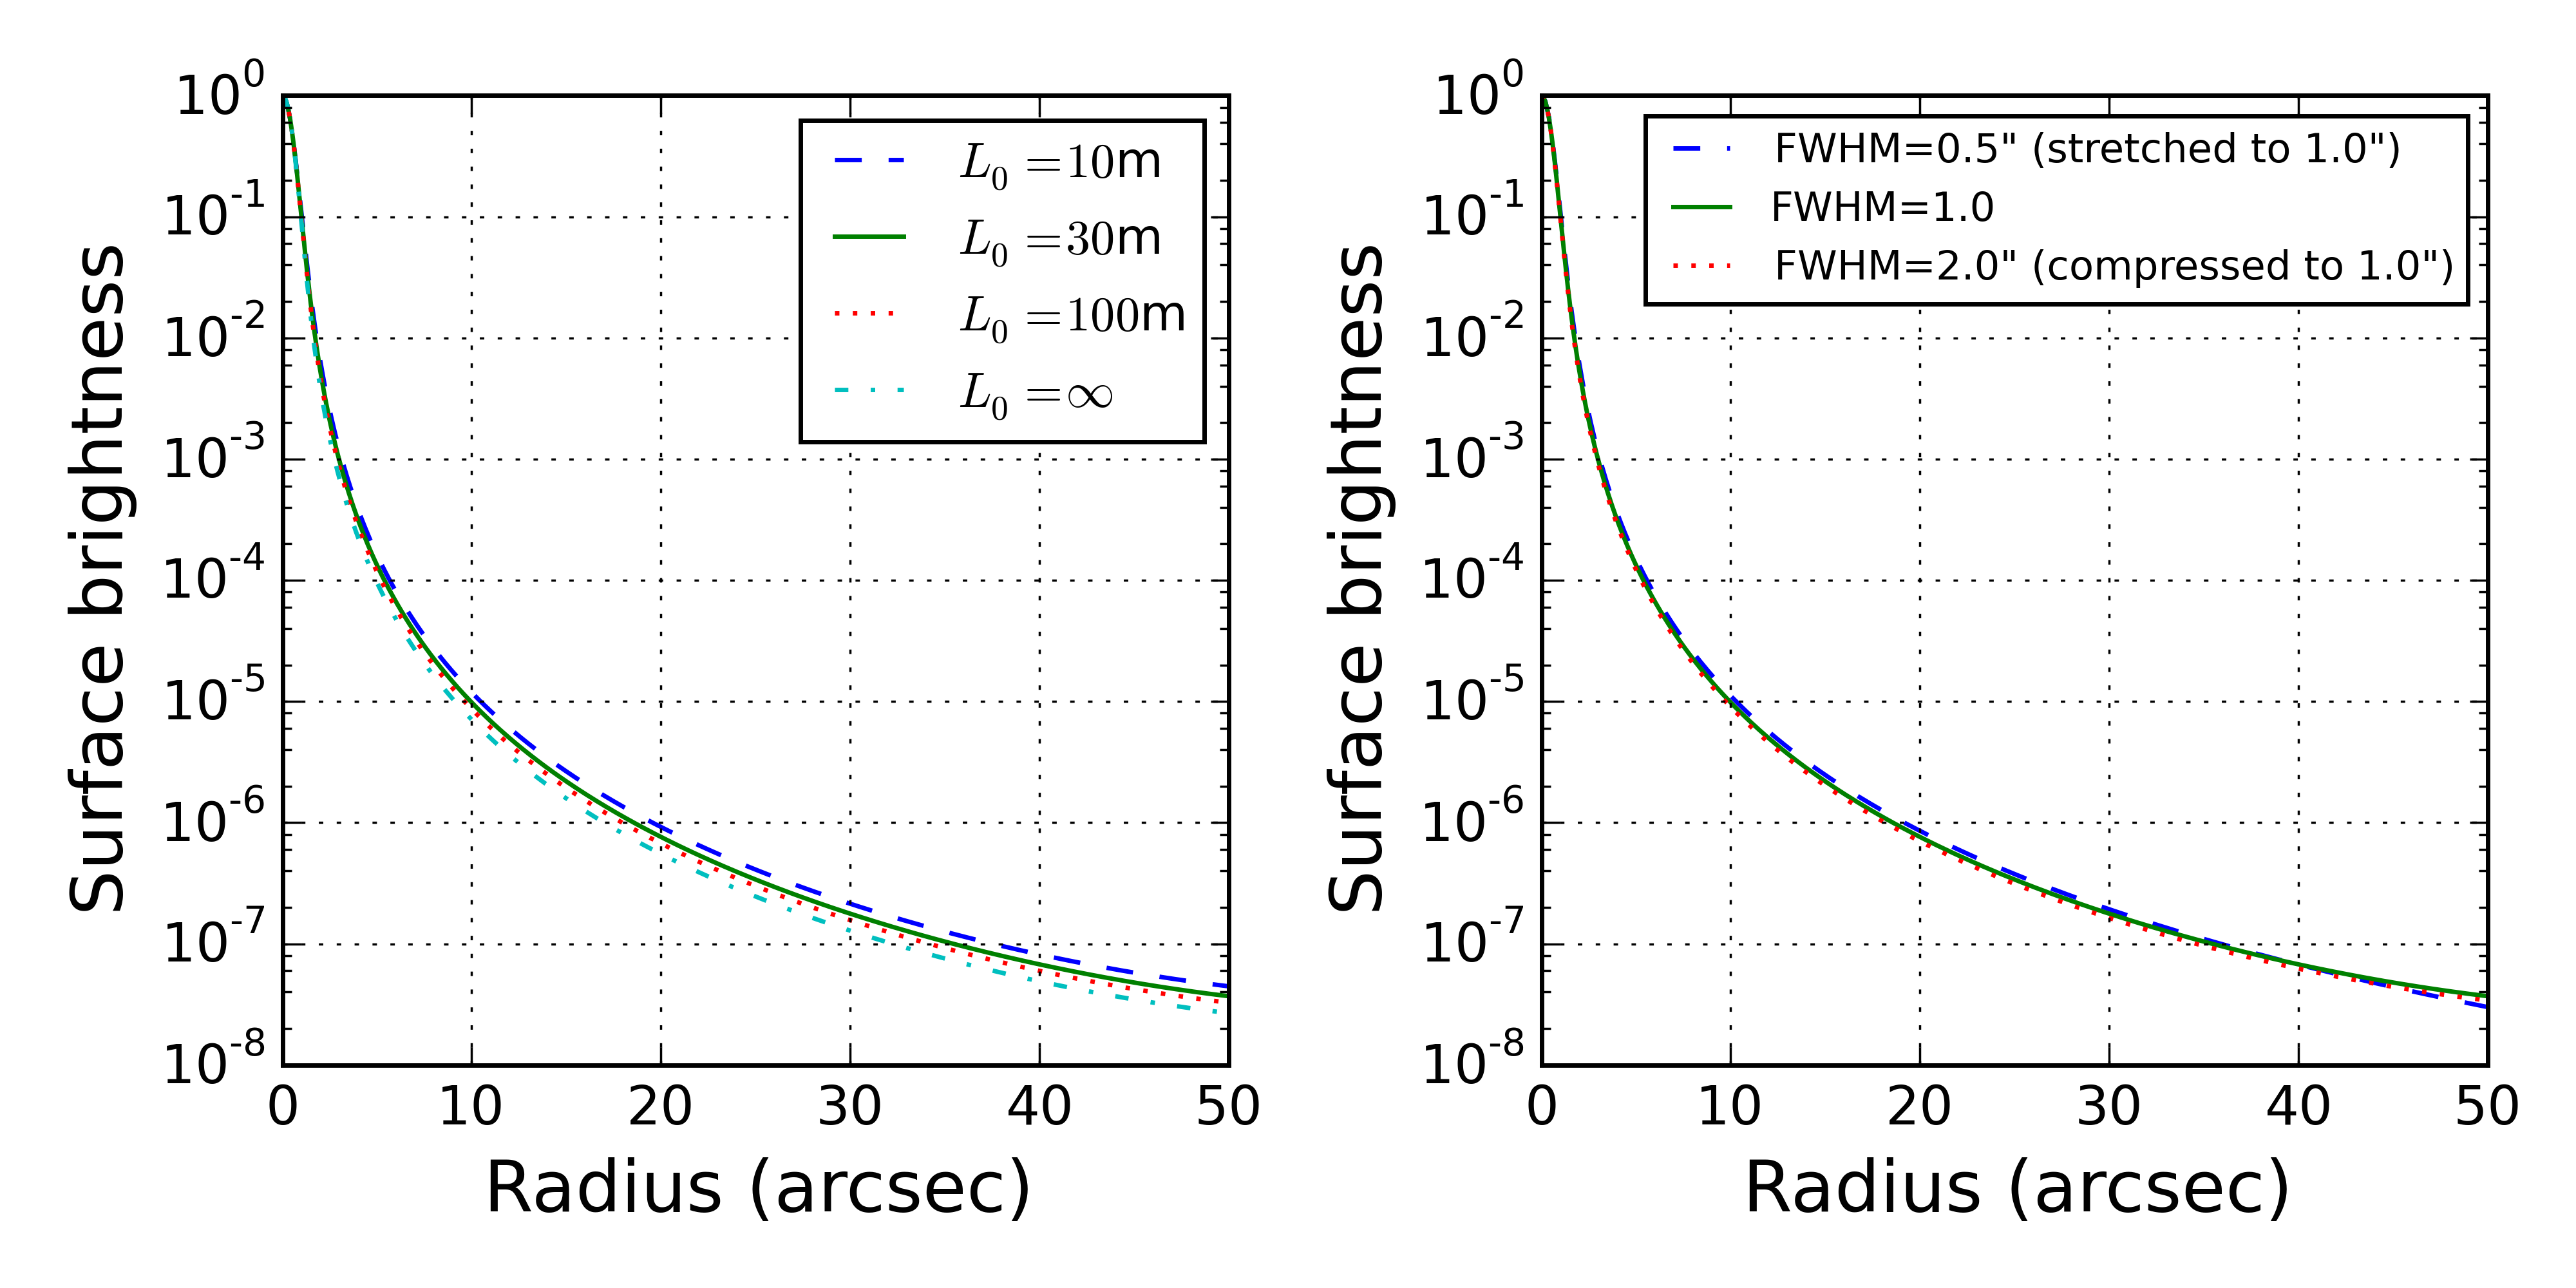
\includegraphics[width=0.8\textwidth]{FIGURES/vonK.png}
\vskip -0.2in 
\caption{PSF radial profiles with the \vk~model for a few different
  outer scale ($L_0$) values (left) and $r_0$ values (right). 
All profiles have FWHM of 1.0 arcsec, and
  are normalized to unit peak intensity. The \vk~model becomes
  Kolmogorov when $L_0 = \infty$.
In the right plot, the dashed and dotted profiles are created with
$L_0 = 30$m, and 
FWHM of 0.5 arcsec and 2.0 arcsec, respectively, then stretched and compressed to 1.0 arcsec.
\label{fig:vonK}}
\end{figure}

The $\chi^2$ is defined using the first four data points on the
measured radial profiles, at 0.16, 0.51, 0.87 and 1.44 arcsec,
respectively. These points correspond to highest photon counts, and 
also are least susceptible to errors in the background brightness
estimates. 
The error estimates on these data points come from the original SDSS measurements.

Although the fitted
curves agree with the input data points very well, generally much better than the
original 6-parameter double-Gaussian fit by SDSS, they do not always describe
the PSF tail beyond $\sim 15$ arcsec radius. 
Some examples of such fits are shown in Fig.~\ref{fig:psffit}.
This discrepancy is easily understood
because the PSF tails in the optical bands can be 
different due to the properties of the CCDs.
The SDSS $u$-, $g$-, $r$-, and $z$-bands differ only slightly due to
changing conversion depth. It is known that the $i$-band PSF has ``stronger tails''
because of scattering in the CCD (J.E. Gunn, priv. comm.). The Si is transparent at long $i$-band wavelengths 
so light goes all the way through the chip and is reflected off the solder, and passes 
back up through the Si. This effect is not visible in the $z$-band because in this case
thick front-side illuminated chips are used (in all other bands, thin back-side chips are used). 



\subsection{Instrumental PSF \label{sec:instrPSF}} 

To improve the fit quality at large radii, in the second fitting step we introduce an
empirical ``instrumental'' PSF. Despite the name, this component might also include 
effects not modeled by the \vk~theory, such as aerosol scattering in the atmosphere,
dust on the mirrors, and scattering in the CCDs. The observed PSF can be expressed 
as a convolution of the atmosphere, represented 
by the \vk, and the instrumental PSF,
\begin{equation}
        \textrm{PSF} = \textrm{vonK} (\textrm{FWHM}) \otimes
        \textrm{PSF}_{\textrm{inst}},
\label{eq:conv}
\end{equation} 
where vonK is the \vk~shape, whose only parameter, FWHM, is fixed to
the value from step one.
Fig.~\ref{fig:psffit} shows that the tails of the PSF can be well
described using a second order polynomial in the logarithmic space of
the intensity.
Meanwhile, since $\textrm{PSF}_{\textrm{inst}}$ is a convolution
kernel, we can use a narrow Gaussian to describe its central core.
We define the functional form of the instrumental PSF as
\begin{equation}
        \textrm{PSF}_{\textrm{inst}} = \exp(-\frac{r^2}{2\sigma^2}) + 10^{p(r)},
\label{eq:psfinst}
\end{equation} 
where $p(r)$ is a second order polynomial.
The standard deviation of the Gaussian, $\sigma$, cannot be
too wide because the \vk~term already well describes the core of the
PSF.
We found that $\sigma = 0.1$ arcsec is an acceptable choice.

We define the second order polynomial $p$ as
\begin{equation}
        p(r) = \eta(ar^2+br+1).
\label{eq:psfinstp}
\end{equation} 
Because the shape of the instrumental PSF tail should not vary with
time, but does vary with the filter and camera column,
we determine the values of $a$ and $b$ for each band-camera-column
combination using one representative
field, then fix them at those values for all step-two fits.
For each SDSS PSF radial profile,
these one-time least-square fits use all the data points with radii up
to $\sim$30 arcsec.
Each fit has $a$, $b$, and $\eta$ as free parameters, and involves a 2-dimensional convolution (see Eq.~\ref{eq:conv}),
The fits are very slow but need to be done only once.
We used here run 94, field 11 for these one-time fits, but verified that 
the results are stable for other choices of run and field. 
The best-fit values of $a$ and $b$ are listed in Table~\ref{tab:abc}.

For step-two PSF fitting, parameters $a$ and $b$ are
fixed for each band-camera-column combination.
$\eta$, the relative normalization of the instrumental PSF
tail in the logarithm-space, is the only free
parameter.
This second fitting step is also a least-square fit with a
2-dimensional convolution, using all the data points
with radii up to $\sim$30 arcsec.
Each two-step PSF fit can be done in a few seconds.
Fig.~\ref{fig:psffit} shows the results of our PSF fits from run 4874. The two-parameter
fits describe the PSF radial profiles quite well, both in the core and
in the tails. The addition of the instrumental PSF 
(dot-dashed lines in Fig.~\ref{fig:psffit})
significantly improves the fit quality, 
especially in the $i$-band. 

Fig.~\ref{fig:psffit} also shows the original SDSS ``double Gaussian plus power-law wing'' fits,
described by Eq.~\ref{eq:SDSSPSF}. They sometimes fail catastrophically; our analysis revealed
two kinds of failures: one case is characterized by $p_0 =10^{-7}$ and
another by $\beta$=3 or 10.
For the sample of 947,400 PSF fits analyzed here, each failure case occurs with a frequency of about 12\%. 
Inspection of the SDSS code (findPsf.c) reveals that these values signal bad fits which did not 
converge for various (unknown) reasons. 

There are a total of 108 runs in the SDSS Stripe 82 dataset. Among them, run 4874 is the longest, 
with 981 fields. In the rest of this paper, whenever we illustrate results from a single run, 
we always use run 4874 as the fiducial example run. 


\begin{figure}[th]
\centering
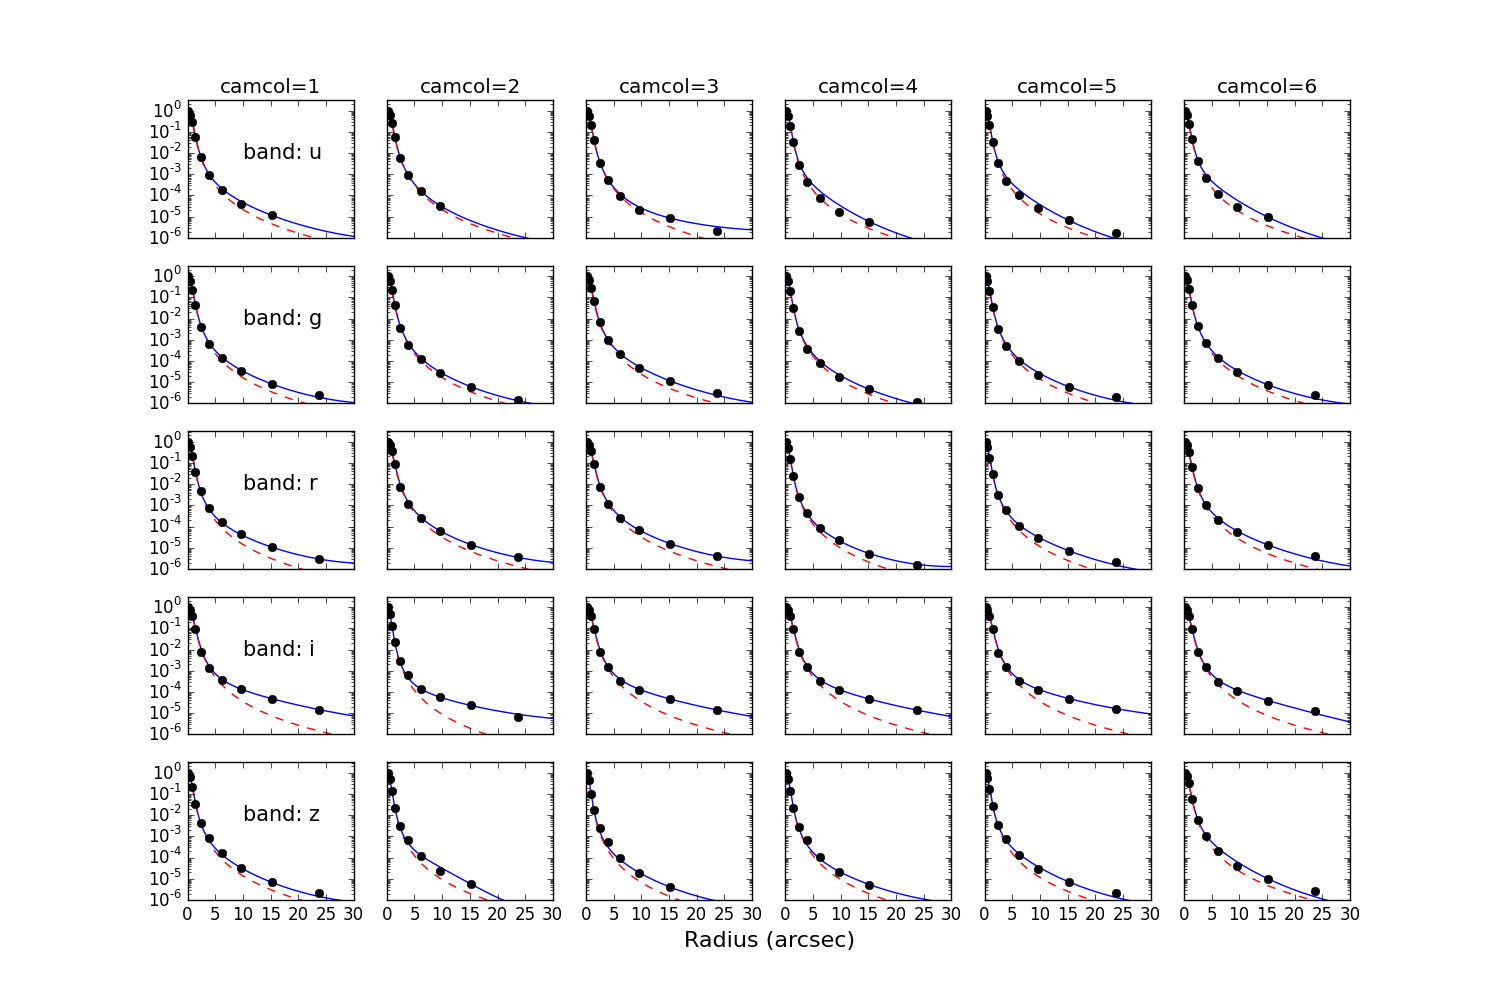
\includegraphics[width=1.0\textwidth]{FIGURES/psffit.png}
\vskip -0.3in
\caption{Fits to the PSF radial profiles from run 4874, field 121. Symbols are SDSS data. 
  Red dashed curves are the best one-parameter \vk~fits. Black solid curves are the red
  curve convolved with the instrumental PSF (green dot-dashed lines), where the scaling factor
  (relative normalization) 
  for the tail component is allowed to vary. 
As a reference, the original ``SDSS double Gaussian plus power-law wing'' fits,
described by eq.~\ref{eq:SDSSPSF}, 
 are shown in blue dotted lines -- they sometimes fail catastrophically (see text). 
Note that the y-axis is shown on the logarithmic scale.
\label{fig:psffit}}
\end{figure}


\begin{table}[th]
\begin{center}
\caption{Values for instrumental PSF shape parameters $a$ and $b$.\label{tab:abc}}
\begin{tabular}{c|c|rrrrrr}
\tableline\tableline
\multicolumn{2}{c|}{} & \multicolumn{6}{c}{Camera Column} \\\cline{3-8}
\multicolumn{2}{c|}{} & 1 & 2 & 3 & 4 & 5 & 6\\\hline
   & a($\times 10^{-4}$) & $-$4.4 & $-$4.4 & $-$1.9 & $-$4.4 & $-$4.4& $-$4.4\\
 $u$& b($\times 10^{-2}$) & 3.3   & 3.3       & 1.3       &      4.7 &4.7   & 4.7\\ \hline
  & a($\times 10^{-4}$) & $-$5.3 & $-$5.3 & $-$4.4 & $-$4.4 & $-$5.3&$-$5.3 \\
 $g$& b($\times 10^{-2}$) & 3.5  & 3.5      & 3.3       &        3.3 &3.5 & 3.5\\\hline
  & a($\times 10^{-4}$) & $-$4.9 & $-$4.9 & $-$4.9 & $-$5.8 &$-$4.4 & $-$4.4\\
 $r$& b($\times 10^{-2}$) & 3.1 & 3.1         & 3.1     &        3.3 &3.3 & 3.3\\\hline
  & a($\times 10^{-4}$) & $-$1.3 & $-$2.2& $-$1.3 & $-$1.3 & $-$1.8& -0.4\\
 $i$& b($\times 10^{-2}$) & 1.7 & 1.8        & 1.7      &        1.7 &1.7 & 1.5\\\hline
  & a($\times 10^{-4}$) & $-$6.2 & 4.4     & $-$6.2 & $-$4.4  &$-$6.2 & $-$4.4\\
 $z$& b($\times 10^{-2}$) & 4.0 & 2.0      & 4.0      &        3.1 &4.4 & 4.7\\
\tableline
\end{tabular}
\end{center}
\end{table}
 

\section{The analysis of FWHM behavior} 


%  \section{The analysis of FWHM behavior} 

Given that the observed seeing is by and large described by a single parameter, FWHM, 
we study three aspects of its variation in detail, as follows.


\subsection{The FWHM dependence on wavelength} 

The Kolmogorov turbulence theory gives a standard formula for the FWHM of a long-exposure
seeing-limited PSF in a large telescope,
\begin{equation}
\textrm{FWHM}^{\rm Kolm}(\lambda, X) = \frac{0.976\lambda}{r_0(\lambda,X)}.
\label{eq:fwhmkolm}
\end{equation}
Here $\lambda$ is the wavelength, $X$ is the airmass, and $r_0$ is the Fried parameter.
We use $\lambda = 500$ nm as the reference wavelength,
\begin{equation}
r_0(\lambda,X) = r_0(500) \left(\frac{\lambda}{500}\right)^{1.2}
\frac{1}{X^{0.6}},
\label{eq:r0}
\end{equation}
where $r_0(500)$ is the $r_0$ for $\lambda=500$ nm and $X$=1, and $\lambda$ is 
expressed in nm.
Substituting Eq.~(\ref{eq:r0}) into (\ref{eq:fwhmkolm}), it is easy to show that 
\begin{equation}
\textrm{FWHM}^{\rm Kolm} \propto \lambda^{-0.2}.
\end{equation}


With the \vk~atmosphere model, the FWHM as in
Eq.~(\ref{eq:fwhmkolm}) needs an additional correction factor
which is a function of the outer scale $L_0$~\citep{Tokovinin2002},
\begin{equation}
\textrm{FWHM}^{\rm vonK}(\lambda, X) = \frac{0.976\lambda}{r_0(\lambda,X)}
\sqrt{1-2.183\left( \frac{r_0(\lambda,X) }{L_0} \right)^{0.356}}.
\end{equation}
If power-law approximation is attempted,  FWHM$^{\rm vonK} \propto \lambda^{\alpha} $, 
$\alpha$ becomes a function of $L_0$ and $r_0$ at a specified
wavelength and airmass, or equivalently, a function of $L_0$ and FWHM$^{\rm vonK}$.
For the subsequent analysis, we adopt the $r$ band as the fiducial band (with
the effective wavelength of 616.6 nm).


\begin{figure}[th]
\centering
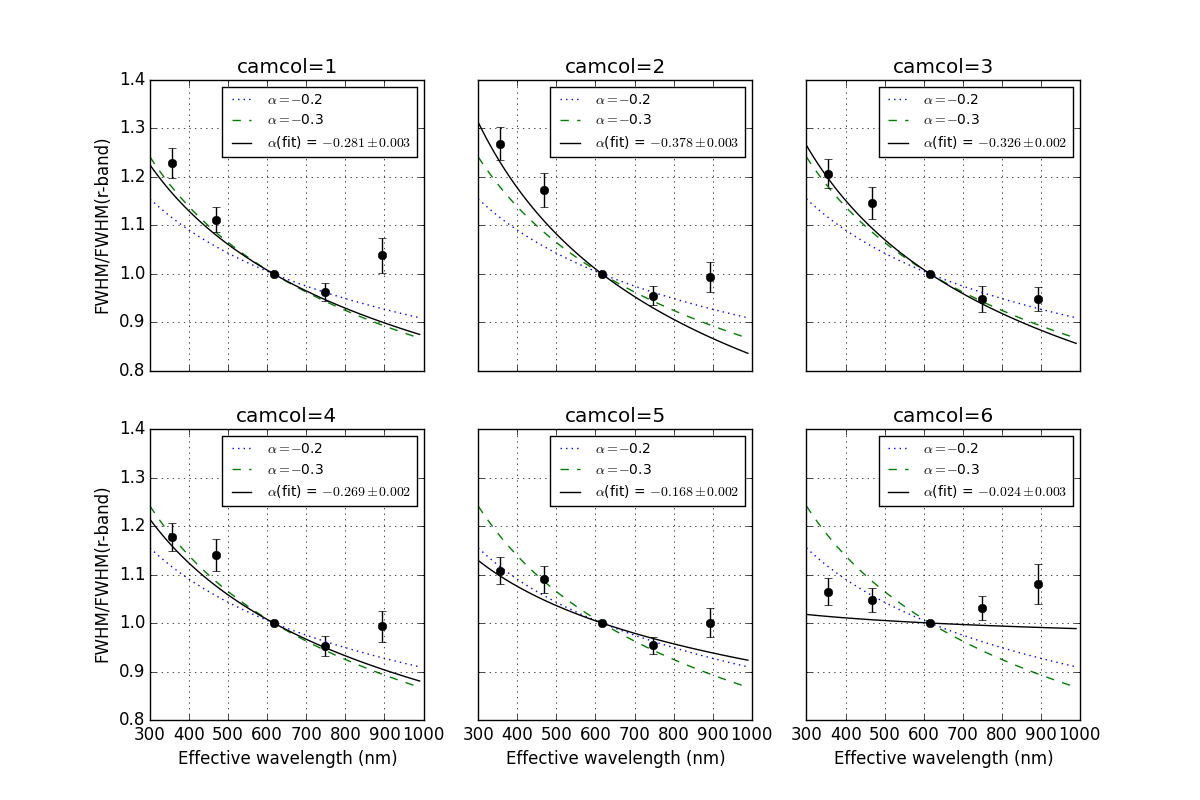
\includegraphics[width=0.9\textwidth]{FIGURES/fwhm_lambda.png}
\caption{The behavior of FWHM as a function of wavelength for the fiducial run 4874.
Symbols are SDSS data and solid line is the best power-law fit, with the best-fit slope
($\alpha$) shown in inset. For comparison purposes, the $\alpha=-0.2$ (dotted) and $\alpha=-0.3$ 
(dashed) lines are also shown. For the ensemble behavior of best-fit $\alpha$, see Fig.~\ref{fig:alpha_fwhm}. 
\label{fig:fwhm_lambda}}
\end{figure}


\begin{figure}[th]
\centering
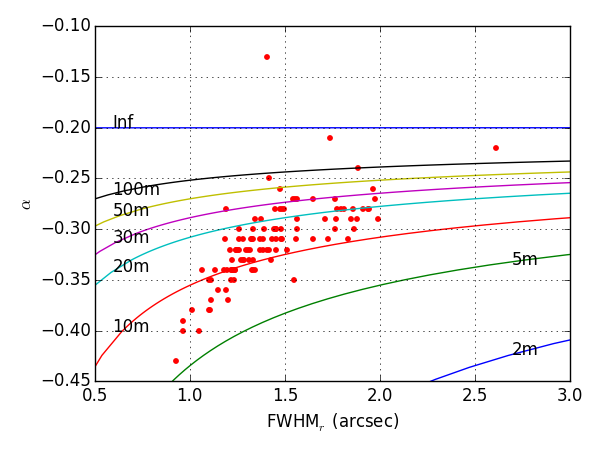
\includegraphics[width=0.8\textwidth]{FIGURES/alpha_fwhm.png}
\caption{The variation of the best-fit power-law index for the wavelength dependence of FWHM, $\alpha$, 
vs. the FWHM in the $r$-band for all the 108 Stripe 82 runs. The symbols are SDSS
measurements in camera column No. 3. The curves are predictions of the 
\vk~model, with $L_0$ ranging from 2 meters to infinity, as labeled. The data are clearly
inconsistent with Kolmogorov predictions ($L_0=\infty$) and reasonably well described by
\vk~model and $L_0$ in the range from 10m to 30m.  \label{fig:alpha_fwhm}}
\end{figure}

 
For each run from SDSS Stripe 82 data, and each camera column, we make
a least-square fit to
all the simultaneous FWHM measurements across the optical bands, to
estimate the power-law index $\alpha$.
All FWHM values are multiplied by $1/X^{0.6}$ to correct for the airmass effects.
We take into account that the same field number does not correspond to the same
time in all filters. The scanning order in the SDSS camera is $r$-$i$-$u$-$z$-$g$, with the delay between the two 
successive filters corresponding to 2 fields. That is, if we take the field number $F$ for the $r$-band, then
we need to take FWHM for the $i$-band from field $F-2$, for the $u$-band
from $F-4$, and so on. 

Fig.~\ref{fig:fwhm_lambda} shows such fits for run 4874. All FWHM are normalized using 
corresponding FWHM in the $r$-band taken at the same moment in time. Significant deviation 
from $\alpha = -0.2$, predicted by the Kolmogorov model, can be seen in most bands.


As discussed above, according to the \vk~atmosphere model, the
power index $\alpha$ should be a function of the outer scale $L_0$ and 
FWHM. 
Fig.~\ref{fig:alpha_fwhm} shows a scatter plot of best-fit $\alpha$ (averaged
over six columns) versus the FWHM in the $r$-band, for all analyzed runs.
A correlation between $\alpha$ and the FWHM seems to be present.
Similar correlations have been seen in Subaru images and reported by~\cite{subaruSeeing2016}.
The data points are overlaid with curves predicted by the 
\vk~model, with $L_0$ varying from 2 m to infinity.
The data clearly deviate from the Kolmogorov model prediction, which is
the horizontal line at $\alpha = -0.20$, with infinite $L_0$.
For example, for LSST's fiducial FWHM of 0.6 arcsec and the commonly assumed 
$L_0 = 30$ m, the \vk~model predicts an $\alpha$ value close to $-0.31$.



\subsection{Angular structure function} 

\begin{figure}[th]
\centering
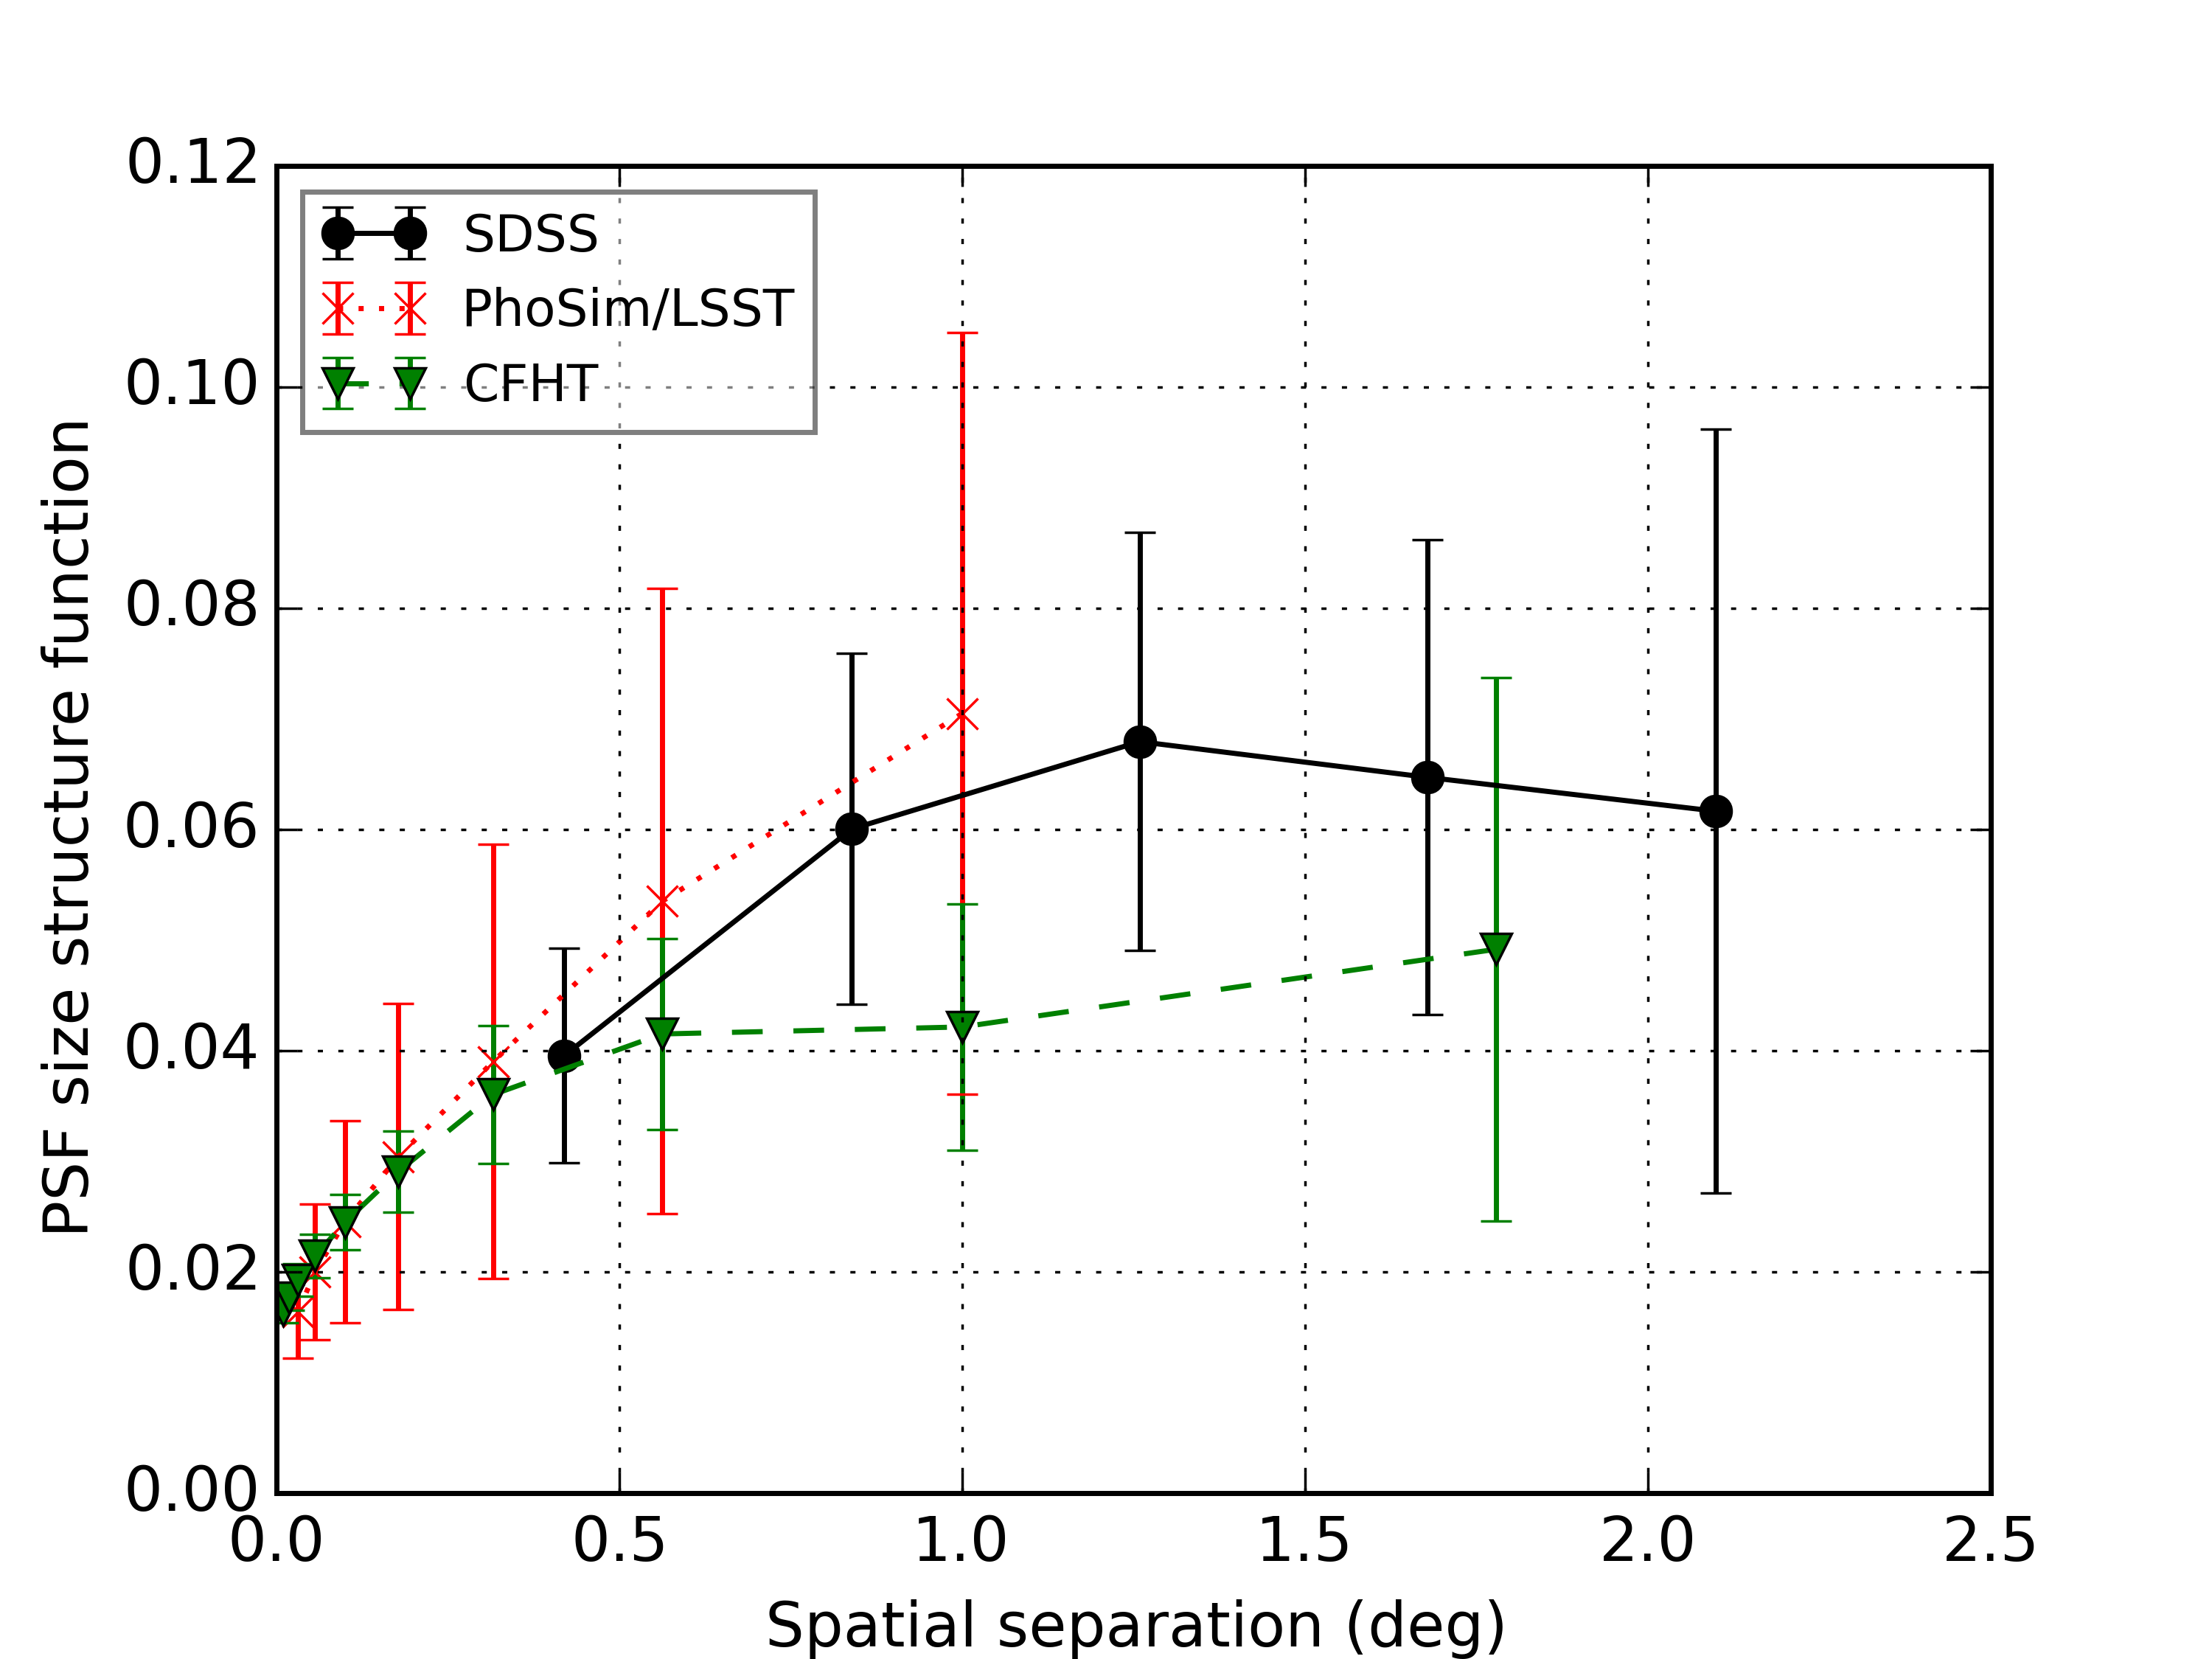
\includegraphics[width=0.8\textwidth]{FIGURES/spatial.png}
\caption{The angular structure function for the PSF size determined using 
  CFHT data from \cite{heymans2012}, SDSS data analyzed here, and LSST image simulations. 
  SDSS measurements are averaged over 86 runs with number of fields larger than 100. 
\label{fig:spatial}}
\end{figure}

To examine the angular (spatial) correlation of the FWHM, we compute the angular
structure function using PSF measurements from all 6 camera columns.
Our structure function is defined as the root-mean-square scatter of the PSF size 
differences of pairs of stars in the same angular bin\footnote{The adopted form 
of the structure function, $SF$, is closely related to the autocorrelation function, $ACF$, as 
$SF \propto (1-ACF)^{1/2}$.} .
The SDSS curves are combined for 86 out of the 108 Stripe 82 runs with the number 
of fields larger than 100.
We also compared the structure functions for each band
separately, and found no statistically significant differences.
Results for the $r$-band are shown in Fig.~\ref{fig:spatial}.

The structure function starts saturating at separations of
$\sim 0.5 - 1.0$ degree, with an asymptotic value of about $\sim 0.05$ arcsec.
In other words, the seeing rms variation at large angular scales is about 5\%,
but we emphasize that our data do not probe scales beyond 2.5 degree. 

For comparison, Fig. ~\ref{fig:spatial} also shows simulated PSF angular
structure functions obtained using PhoSim~\citep{phosim},
and results from the CFHT PSF measurements~\citep{heymans2012}.
The PhoSim PSF profiles are obtained by simulating a grid of stars
spaced by 6 arcminutes with non-perturbed LSST telescope and ideal sensors.
The results are averaged over 9 different atmosphere realizations with
different wind and screen parameters and airmass, and over 3 different
wavelengths (350 nm, 660 nm, and 970 nm).
The CFHT PSF size measurements were made in the $i$-band, and provided
by the authors of~\cite{heymans2012}.
The three curves in Fig.~\ref{fig:spatial} appear to be quantitatively
consistent with each other, even though they correspond to telescopes at
different sites and with different optics.


\subsection{Temporal behavior}

\subsubsection{Power spectrum analysis} 

\begin{figure}[th]
\centering
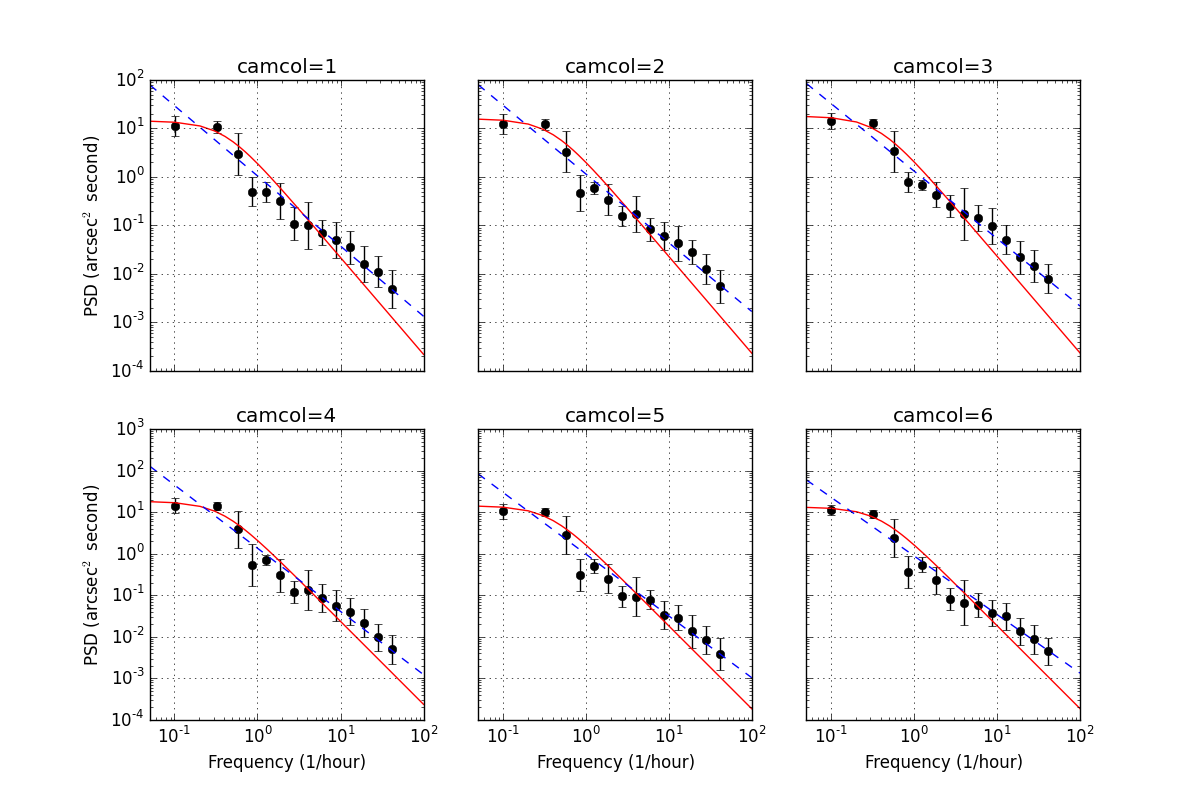
\includegraphics[width=0.99\textwidth]{FIGURES/temporalPSD.png}
\vskip -0.2in
\caption{PSF size temporal power spectral density for run 4874, r-band. 
The solid lines are fits using the damped random walk model. 
The dashed lines show best fits based on a single power law. The former
predicts a steeper high-frequency behavior, while the latter cannnot 
explain the turnover at low frequencies. 
\label{fig:psd}}
\end{figure}

To study the temporal behavior of the seeing, we first analyze its power spectrum.
Fig.~\ref{fig:psd} shows the temporal power spectral density (PSD) of the
PSF FWHM for 6 camera columns, in run 4874, $r$-band.
The time difference between subsequent fields is 36 seconds.
We fit the PSD using two competing models.
The first is a damped random walk (DRW) model~\citep[for introduction see Chapter 10 in][]{zeljkoBook},
\begin{equation}
\textrm{PSD}(f) = \frac{\tau^2 SF^2_{\infty}}{1+(2\pi f \tau)^2},
\end{equation}
where $f$ is the temporal frequency, $SF_{\infty}$ is the asymptotic
value of the structure function, and $\tau$ is the
characteristic timescale.
The solid curves in Fig.~\ref{fig:psd} show fits using this model.
Note that due to the lack of data toward the low-frequency end, the
first and second bins are four and two times wider than the
rest of the bins, respectively.
Combining fit results for all camera columns and optical bands for run 4874
gives $\tau = 23.6 \pm 1.3$ minutes.
Making the same fits for all the 108 runs in Stripe 82, 
we obtain the $\tau$ distribution vs. the duration of each
run, as shown in Fig.~\ref{fig:hist} (left).
The shorter runs tend to give smaller timescale. It is plausible that short runs 
cannot reliably constrain $\tau$ due to the lack of data toward the low-frequency 
end of the spectra. There are 12 runs longer than 6 hours and their characteristic timescales
are within the range of about $\sim10-30$ minutes.
This results is generally consistent with ~\cite{Racine1996}, where a timescale of 
$\tau = 17 \pm 1$ minutes was found.

The data consistently show a shallower high-frequency behavior than predicted
by damped random walk ($\propto 1/f^2$). In order to quantitatively describe 
the high-frequency tail of the PSD, we fit a simple power law,
\begin{equation}
\textrm{PSD}(f) = B f^\beta,
\end{equation}
where $B$ is the normalization factor, and $\beta$ is the power-law index.
Best-fits are illustrated for run 4874 are in Fig.~\ref{fig:psd} (dashed lines).
Combining fit results for all camera columns and filters gives $\beta = -1.29\pm 0.09$ 
for run 4874. Making the same fits for all the 108 runs in Stripe 82, we obtained the 
$\beta$ distribution vs. the duration of each run shown in Fig.~\ref{fig:hist} (right).
The shorter runs give $\beta$ values with a larger variance, but nevertheless it is 
clear that for most runs the high-frequency behavior can be described with a 
power-law index in the range $-1.5$ to $-1.0$. On the other hand, a single 
power law cannot explain the turnover at low frequencies. 

Therefore, neither model provides a satifactory fit over the entire frequency range: 
the power law fit systematically over predicts the low-frequency part of the PSD,
while the $1/f^2$ high-frequency behavior of damped random walk model is too 
steep. It is likely that a hybrid model would work, but we leave detailed analysis
for future work. 


\begin{figure}[th]
\centering
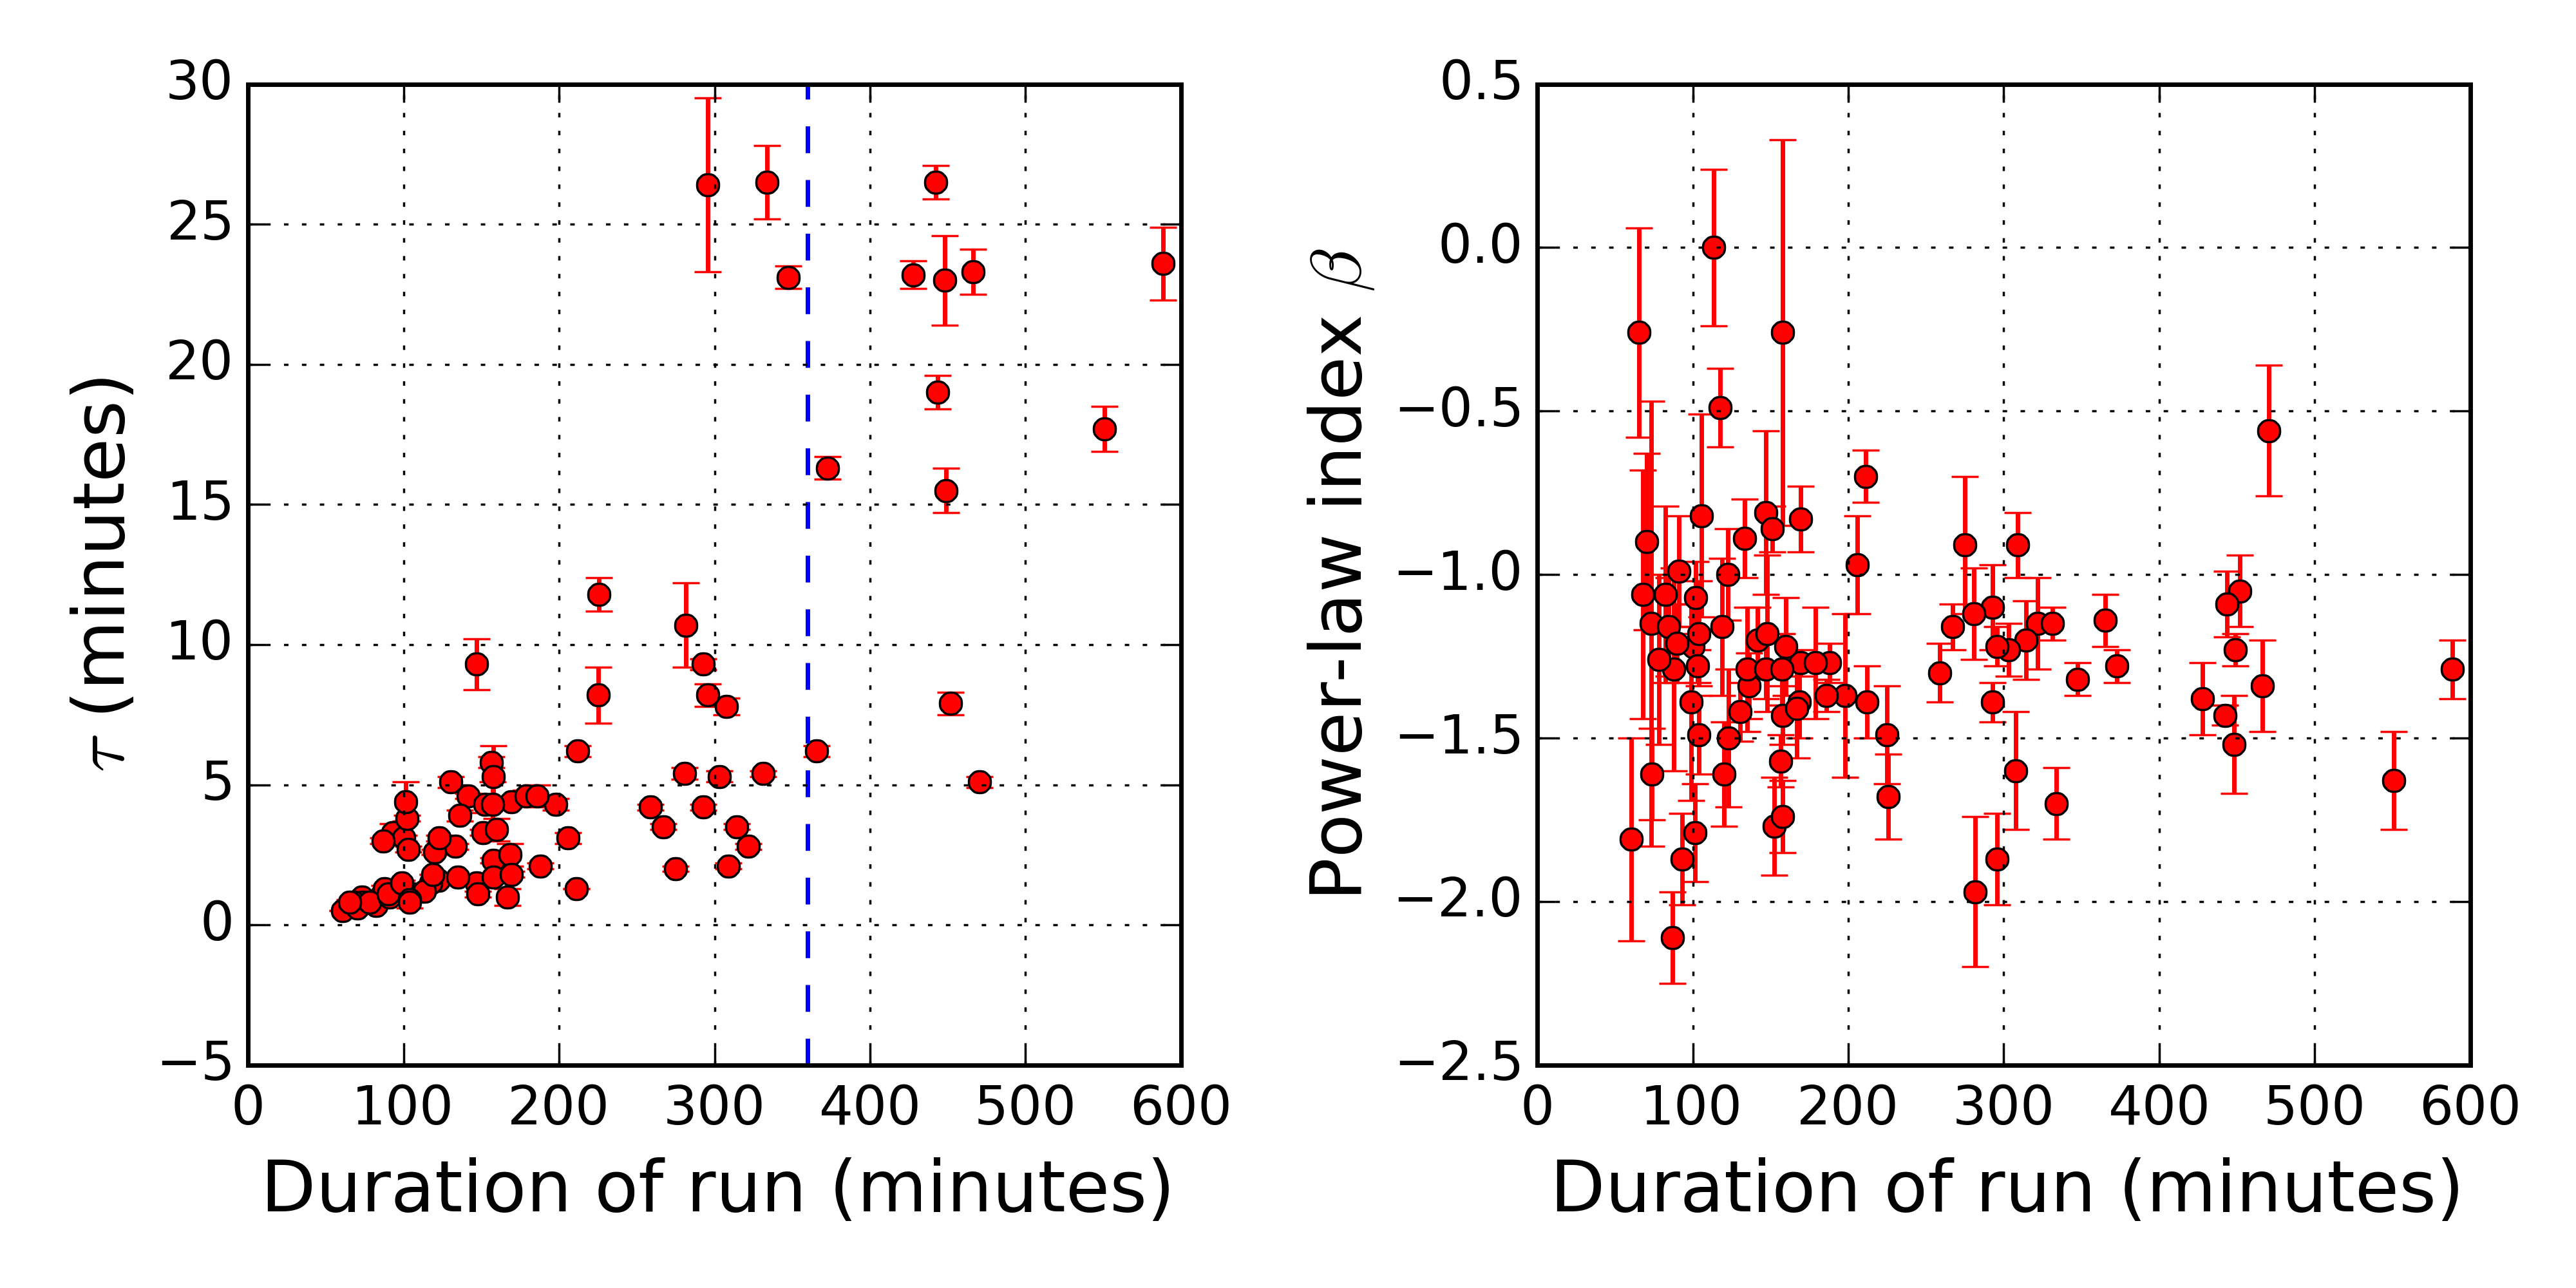
\includegraphics[width=0.99\textwidth]{FIGURES/taubeta.png}
\vskip -0.2in
\caption{Left: The symbols show the best-fit characteristic timescale $\tau$ in 
damped random walk for all 108 runs in Stripe 82 vs. the duration of 
each run. It is plausible that short runs cannot reliably constrain $\tau$.
Right: The power-law index $\beta$ for a single power law fit for all 108 
runs vs. the duration of each run. Note that for the majority of runs, $\beta$
is larger than the value appropriate for damped random walk ($\beta = -2$). 
\label{fig:hist}}
\end{figure}



\subsubsection{Structure function analysis} 


\begin{figure}[th]
\centering
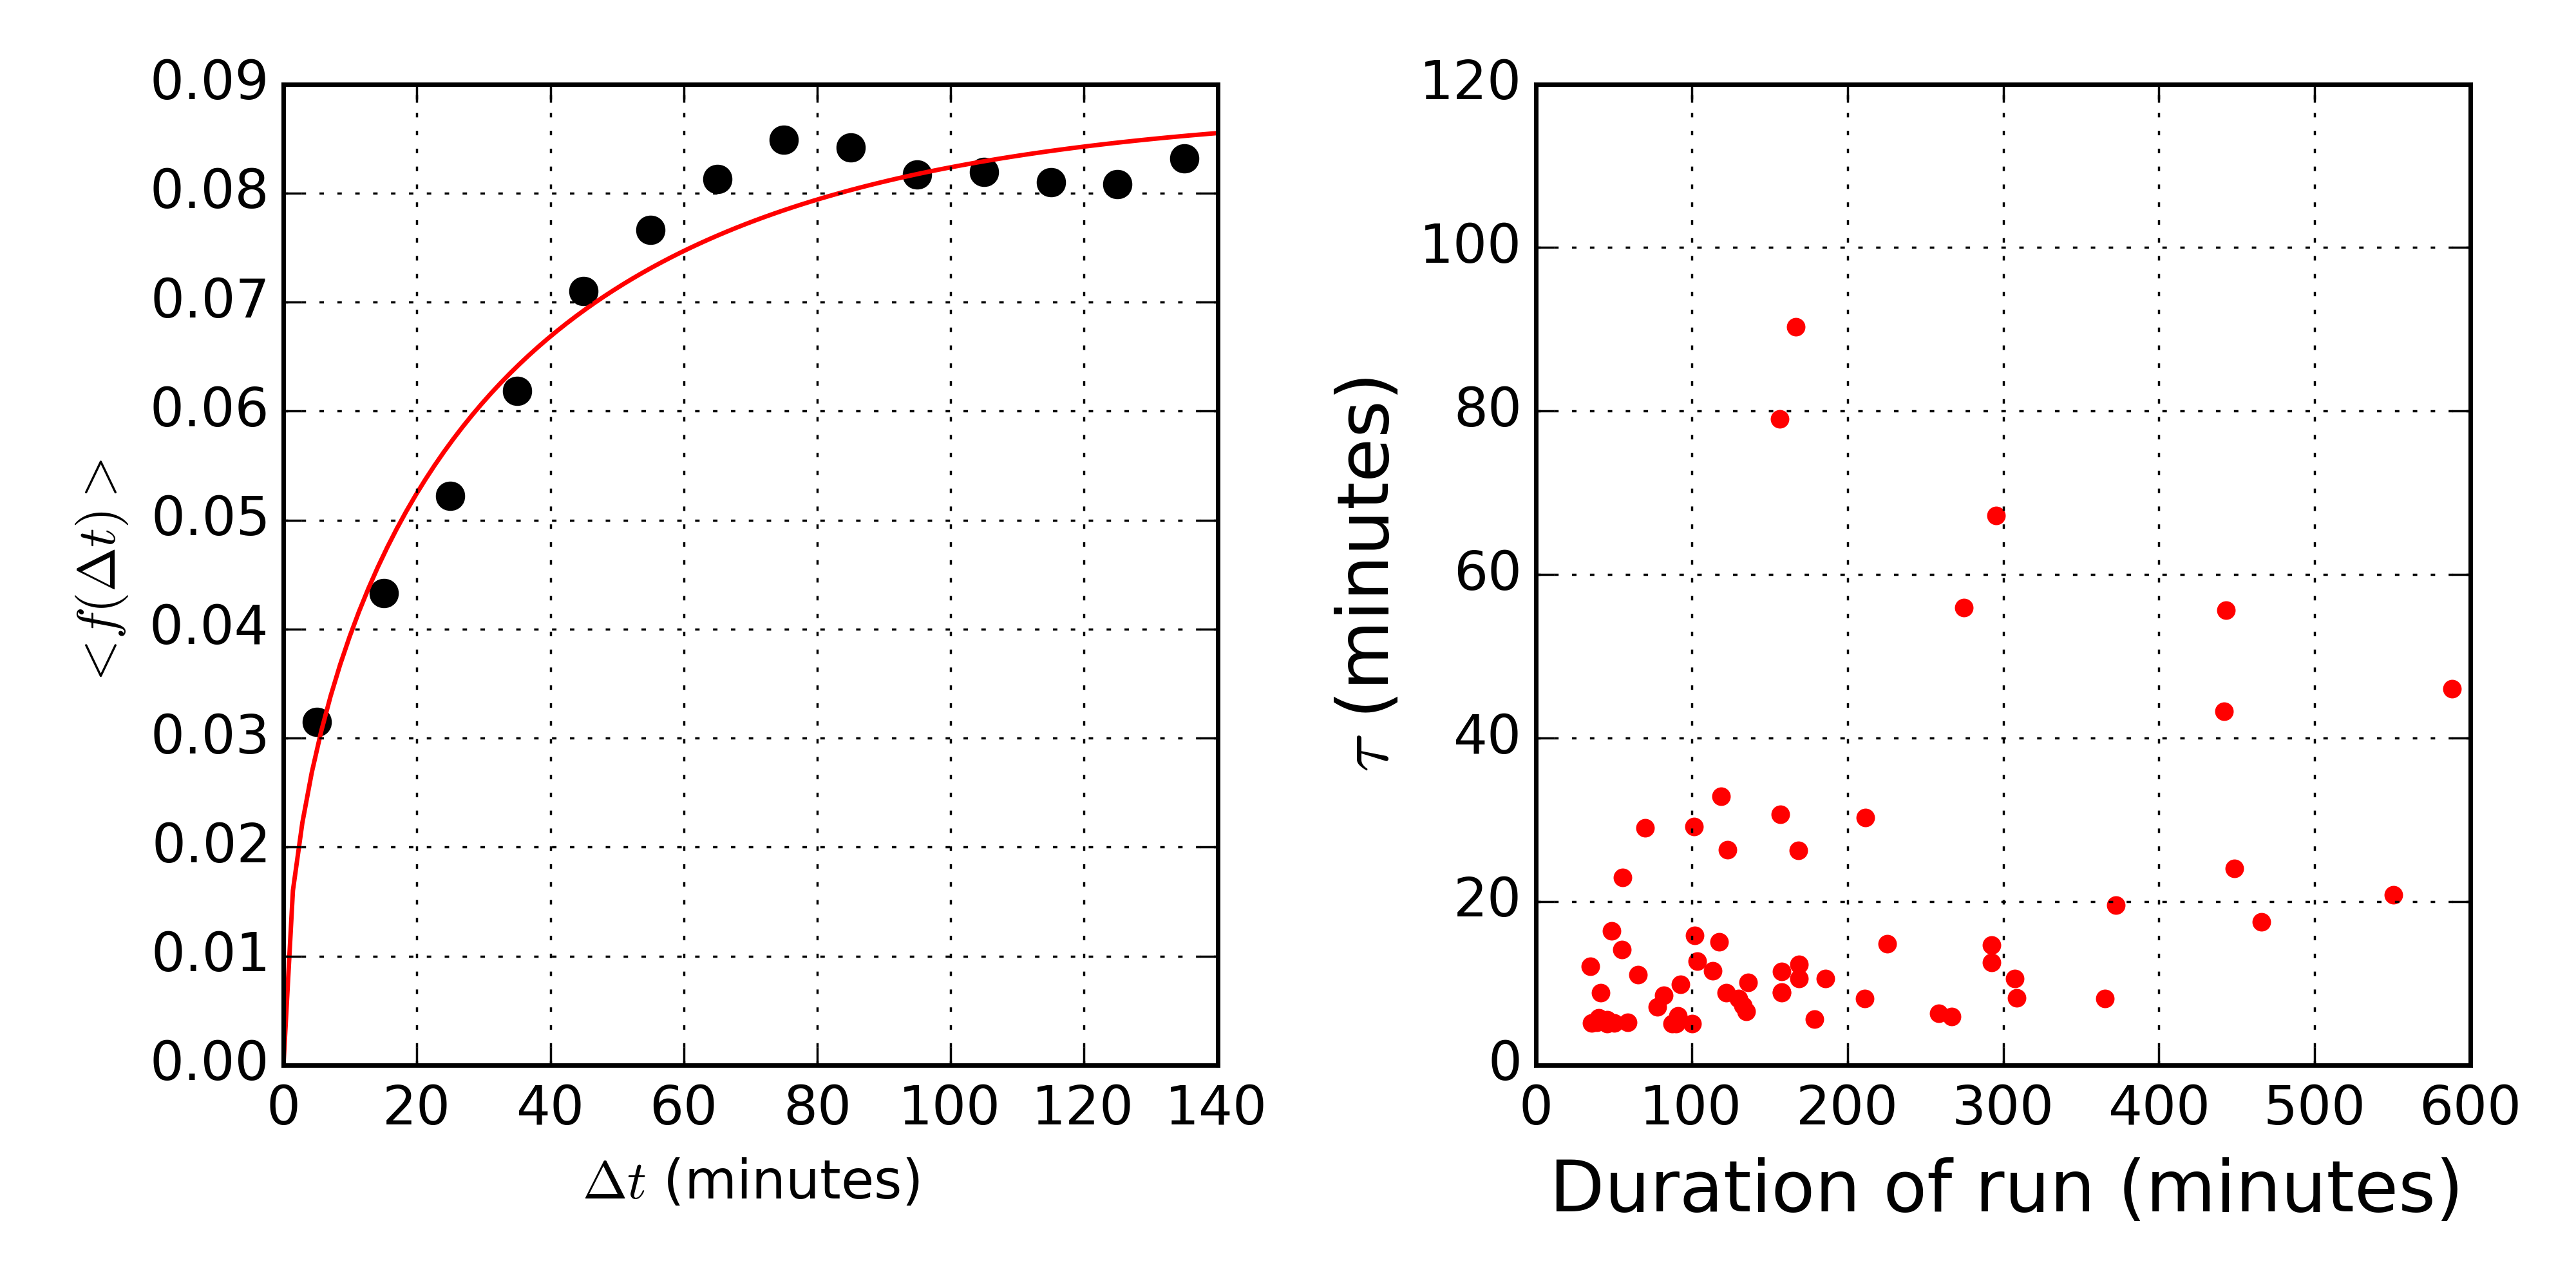
\includegraphics[width=0.9\textwidth]{FIGURES/fdt.png}
\caption{Left: The average normalized seeing difference, $<f(\Delta t)>$, as
  a function of the time separation, $\Delta t$, for run 4874, camera
   column 1, in the $r$-band. The fit to Eq.~(\ref{eq:fdt}) gives $f(\Delta t) ^\infty =  
   0.08$, $\tau = 25.9$ minutes and $\gamma$ = 1.49. The dashed line is the 
   structure function predicted by damped random walk model with the same 
   $f(\Delta t) ^\infty$ and $\tau$. 
Right: The timescale $\tau$ for all 108 runs vs. the duration of each run.
 Note that for most runs $\tau$ is in the range 10-30 minutes
    ($\tau$ is set to zero for runs shorter than 20 minutes).  
\label{fig:fdt}}
\end{figure}


An alternative approach to power spectrum analysis is offered by auto-correlation 
and structure function analysis. Following~\cite{Racine1996}, we define a 
structure-function-like quantity
\begin{equation}
       f(\Delta t) = {| \theta(t+\Delta t) - \theta(t)| \over  \theta(t+\Delta t) + \theta(t) },
\end{equation} 
where $\theta$ is seeing. We then fit the mean value of $f(\Delta t)$ to 
\begin{equation}
    < f(\Delta t) > =  f(\Delta t) ^\infty \, \left[ 1 - \exp(-(\Delta
      t/\tau)^\gamma) \right]^{1/2},
\label{eq:fdt}
\end{equation} 
with $f(\Delta t) ^\infty$, $\tau$ and $\gamma$ as free parameters.
Fig.~\ref{fig:fdt} (left) shows one example of such fits. This functional form is 
somewhat inspired by damped random walk model, where $\gamma=1$ and the 
term in brackets is raised to the power of a half. For illustration, Fig.~\ref{fig:fdt} 
also shows a damped random walk model fit with the same $f(\Delta t) ^\infty$
and $\tau$. 

The best-fit $\gamma$ is found to be mostly in the range 1.0 -1.5. 
The distribution of $\tau$ vs. 
the duration of each run is shown in Fig.~\ref{fig:fdt} (right) (somewhat 
arbitrarily, we set $\tau$ to zero for runs shorter than 20 minutes).  
While the short runs show a larger variance in $\tau$, it is evident that 
for most runs the timescale $\tau$ is in the range 10-30 minutes.
Therefore, this analysis seems more robust at constraining the characteristic time
scale than fitting a damped random walk model to empirical PSD. 
 

\section{Discussion and Conclusions} 


%  \section{Discussion and Conclusions} 
 
For now, a collection place for stuff from other seeing papers (commented out),
and some text to move later to Sections 3 and 4. 


1) \cite{VMT1998} 

For seeing prediction, it is tempting to find statistical laws which describe its temporal behaviour.
To our knowledge only three authors (Racine, 1996; Munoz-Tunon et al., 1997; Sarazin, 1997) 
have worked on this problem. 

- fig. 2: average autocorrelation function of seeing over 9 months:  A*exp(-t/tau) 

- seeing distribution is  log–normal, due to the fact that seeing arises from the addition of uncorrelated random processes


with $\tau$=17 min and $\gamma \sim 0.7$. for observations at Mauna Kea \cite{Racine1996}

Seeing varies greatly with time and seems to decorrelate after 1 to 2 hr. 

The seeing auto-correlation function
\begin{equation}
      C(\Delta t) = < \theta(t) \theta(t+\Delta t)>,
\end{equation} 
can be modeled as
\begin{equation}
      C(\Delta t) = A \, \exp(-\Delta t/\tau),
\end{equation} 
with $\tau \sim 1$ hour. 
 
Triple correlation:
\begin{equation}
      C(\Delta t_1, \Delta t_2) = < \theta(t) \theta(t+\Delta t_1)\theta(t+\Delta t_2) >
\end{equation} 

2) 

The vertical distribution of the optical turbulence strength (energy profile), described by the altitude 
dependence of the refractive-index structure constant $C^2_n$, is hard to measure. When $C^2_n$ 
is available, the seeing $\theta$ is obtained by integrating $C^2_n$ over altitude $h$ as 
\begin{equation}
   \theta =  0.98 {\lambda \over r_0} = 5.25 \, \lambda^{-1/5} \, \left[ \int_0^\infty C_n^2(h) dh \right]^{3/5},
\end{equation}
where $r_0$ is the Fried's parameter \cite{Roddier1981}. 






% Statistics of turbulence profile at Cerro Tololo: 
%A. Tokovinin, S. Baumont and J. Vasquez
%Mon. Not. R. Astron. Soc. 340, 52–58 (2003)

%the Gemini site testing campaign at Cerro Pachon (Vernin et al. 2000; Avila et al. 2000)
%http://www.gemini.edu/documentation/webdocs/rpt/rpt-ao-g0094-1.ps
% SPIE: 
%http://proceedings.spiedigitallibrary.org/proceeding.aspx?articleid=898738

% Coulman (1985, ARAA 23, 19) for theory of turbulence and seeing in astronomy

\begin{equation} 
FWHM = 0.98 {\lambda \over r_0} 
\end{equation} 
where $\lambda$ is the wavelength and $r_0$ is the Fried's
parameter. It can be shown that the variation of $r_0$ with wavelength
predicted by the Kolmogorov's turbulence implies $FWHM \propto \lambda^{-0.2}$. 	
% cite: Vernin, J.; Munoz-Tunon, C. 1992, Astronomy and Astrophysics, vol. 257, no. 2, p. 811-816. 

% Check for seeing forecastas and "flexible scheduling" !! 
% http://www.sciencedirect.com/science/article/pii/S1387647398000438
% also
% The temporal behaviour of seeing:
% Using a large amount of data gathered during previous seeing campaign
% at ORM, we analyse the temporal evolution of seeing in order to find
% out whether predictions could be made over a short time interval of a
% few hours. The first results are presented.
% http://www.sciencedirect.com/science/article/pii/S1387647398000517

% time dependence of seeing: http://adsabs.harvard.edu/abs/2001BASI...29...39S
% they give references for time scales (from 15 mins to 2 hours), also
% see a claim for 2 hour time scale:
% http://adsabs.harvard.edu/abs/2003A%26A...409.1169T
% TMT testing - seeing:
% http://adsabs.harvard.edu/abs/2009PASP..121.1151S 
% HSC seeing in V and K: bad seeing has flatter seeing vs. lambda due
% to outer scale effects
% http://adsabs.harvard.edu/abs/2016ExA....42...85O

% a good summary of work to date for introduction
% https://arxiv.org/pdf/1206.3319.pdf

% forecasting "These characteristics make forecasting seeing a tall challenge."
% http://adsabs.harvard.edu/abs/2015JPhCS.595a2029R
% but this one claims some success using ARIMA:
% http://adsabs.harvard.edu/abs/2016ExA....41..223K 


\acknowledgments




%% To help institutions obtain information on the effectiveness of their
%% telescopes, the AAS Journals has created a group of keywords for telescope
%% facilities. A common set of keywords will make these types of searches
%% significantly easier and more accurate. In addition, they will also be
%% useful in linking papers together which utilize the same telescopes
%% within the framework of the National Virtual Observatory.
%% See the AASTeX Web site at http://aastex.aas.org/
%% for information on obtaining the facility keywords.

%% After the acknowledgments section, use the following syntax and the
%% \facility{} macro to list the keywords of facilities used in the research
%% for the paper.  Each keyword will be checked against the master list during
%% copy editing.  Individual instruments or configurations can be provided 
%% in parentheses, after the keyword, but they will not be verified.

{\it Facilities:} \facility{SDSS}, \facility{LSST}.

%% Appendix material should be preceded with a single \appendix command.
%% There should be a \section command for each appendix. Mark appendix
%% subsections with the same markup you use in the main body of the paper.

%% Each Appendix (indicated with \section) will be lettered A, B, C, etc.
%% The equation counter will reset when it encounters the \appendix
%% command and will number appendix equations (A1), (A2), etc.

%\appendix
%
%\section{Appendix material}

%% The reference list follows the main body and any appendices.
%% Use LaTeX's thebibliography environment to mark up your reference list.
%% Note \begin{thebibliography} is followed by an empty set of
%% curly braces.  If you forget this, LaTeX will generate the error
%% "Perhaps a missing \item?".
%%
%% thebibliography produces citations in the text using \bibitem-\cite
%% cross-referencing. Each reference is preceded by a
%% \bibitem command that defines in curly braces the KEY that corresponds
%% to the KEY in the \cite commands (see the first section above).
%% Make sure that you provide a unique KEY for every \bibitem or else the
%% paper will not LaTeX. The square brackets should contain
%% the citation text that LaTeX will insert in
%% place of the \cite commands.

%% We have used macros to produce journal name abbreviations.
%% AASTeX provides a number of these for the more frequently-cited journals.
%% See the Author Guide for a list of them.

%% Note that the style of the \bibitem labels (in []) is slightly
%% different from previous examples.  The natbib system solves a host
%% of citation expression problems, but it is necessary to clearly
%% delimit the year from the author name used in the citation.
%% See the natbib documentation for more details and options.


\bibliographystyle{aj}
\bibliography{sdsspsf}


%% The following command ends your manuscript. LaTeX will ignore any text
%% that appears after it.

\end{document}

%%
%% End of file `sample.tex'.

----------Completed: ----------------

ZI:  find exact definition of neff_psf (is it based on fit or input data?) 
Bo: add analysis directory and py code 


1)  make files, one per run, as a function of field number, with
- field, camera column, bandpass, 
- one-parameter fit FWHM from fitting von Karman profile
- other SDSS params: psf_width, airmass, mjd, psf_nstar, neff_psf, sky_frames 


E.g. for some run
#  field  camCol  filter   FWHMvK    (other SDSS params)

2) plot FWHMvK vs. psf_width for 30 panels 

-----use a Gaussian as convolution kernel, remake fits -------

Bo:
check neff_psf from the vK fit and compare to 2G fit.
(checked fwhmeff, i.e., fwhmvk, and compared to psf_width from the 2G
fit. Generally the agreement is good. When they don't agree very well,
visually checking the vK fit vs the 2G fit shows that the vK fit often
gives the more reasonable agreement between data and fit.)
------make RMS (x - data) plots to quantify -----------
            /n(-1?) for 1-4, 5+ separately
            exclude bad 2G fits

3) plot alpha (index for lambda dep.) histograms for all data and for 
    two realizations of ``longest stretch'' selection
(not very conclusive, due to z-band tipping upward. The i-band could
be problematic too)

----------to do ----------------

---alpha vs seeing, col#6, col#3
??? masterTXT, a column to flag failed 2D fits?
???(in the master txt file for alpha, add seeing as a column)

4) plot profiles for a range of fields when the seeing is rapidly changing (is profile shape changing?) 


-------------Analysis structure: -----------------

1) profile discussion
- compare to SDSS, emphasize 1 parameter vs. 6 parameters
- discuss profile shape stability when seeing is changing rapidly

2) dependence on wavelength

- what is alpha distribution? 

3) cross-correlation of camera columns and measurement of structure function
    (that is, the covariance vs. angular distance) 

---for each run, each filter, make plot of cov vs separation
----fit through (0,1), plot slope as a function of seeing

4) auto-correlation function (and power spectrum) for temporal variation

- let's start with plain Fourier transform and look at power spectra (we can 
    play games with co-addition, 6 columns for a given run, or all runs)
- potentially, we could also look at  Kelly and Becker code  (2014, ApJ 788, 33) 
- here we can compare to Chuck's CP measurements (in opsim db) 

---for each run, each filter, camcol (#2,3), make D vs frequency.


Adaptive Beaming and Imaging in the Turbulent Atmosphere 
by Vladimir P. Lukin; Boris V. Fortes, Chapter 3, SPIE Press Book.
Fig 3: the depdendence of FWHM on D, Lo and lambda 




FWHM vs. field analysis

1040: 122 fields, oscillations on 5 min timescale, look at PSD 
2583: 227 fields, excellent seeing (1.1 in r) 
2662: 469 fields, long with typical seeing, with worst at the end
2709: 263 fields, oscillations on 5 min timescale, look at PSD 
2728: 488 fields, long with good seeing (1.2 in r) 
3325: 493 fields, long with typical seeing, with worst at the start
3360: 513 fields, typical but very variable seeing
3384: 784 fields, a long and *very* oscillatory run
3388: 713 fields, very different PSD than for 3384 
4145: 505 fields, steady deterioration from 1 arcsec to ~2 arcsec
4198: 747 fields, another long run with typical and oscillatory seeing
4203: 777 fields, another long run
4207: 753 fields, another long run
4849: 918 fields, a long run, typical seeing 
4868: 609 fields, another long run
4874: 981 fields, the longest run, typical seeing   *poster child* 


I would exclude runs with fewer than 100 fields from our analysis 